\documentclass{beamer}
%\usepackage[T1]{fontenc}
\usepackage[utf8]{inputenc}
%\usepackage{lmodern}  % Use the Latin Modern font family

\usepackage{latexsym,amsmath,xcolor,bm, amssymb, color, tikz, graphicx, amsthm, mathtools}
\usepackage{algorithm}
\usepackage{algorithmic}
\usepackage{hyperref}
\usepackage{float}     
\usepackage{CJKutf8}
\usepackage{multicol}

\DeclareMathOperator*{\argmax}{arg\,max}
\DeclareMathOperator*{\argmin}{arg\,min}
\DeclareMathOperator{\sign}{sign}
\DeclareMathOperator{\Tr}{Tr}

\makeatletter
\DeclareRobustCommand\onedot{\futurelet\@let@token\@onedot}
\def\@onedot{\ifx\@let@token.\else.\null\fi\xspace}
\def\eg{\emph{e.g}\onedot} 
\def\Eg{\emph{E.g}\onedot}
\def\ie{\emph{i.e}\onedot} 
\def\Ie{\emph{I.e}\onedot}
\def\cf{\emph{c.f}\onedot} 
\def\Cf{\emph{C.f}\onedot}
\def\etc{\emph{etc}\onedot} 
\def\vs{\emph{vs}\onedot}
\def\wrt{w.r.t\onedot} 
\def\dof{d.o.f\onedot}
\def\etal{\emph{et al}\onedot}
\makeatother


\usetheme{Madrid}
\useinnertheme{circles}


\definecolor{ColorUNR}{HTML}{0b2755} 
\usecolortheme[named=ColorUNR]{structure}
%\usecolortheme[named=ColorUNR]{exampleblock}

%\setbeamertemplate{blocks}[rounded][shadow=true]
%\setbeamercolor{block body}{fg=black,bg=white}



%------------------------------------------------------------
%This block of code defines the information to appear in the
%Title page
\title %optional
{Bienvenidos al Training Camp 2025}

%\subtitle{(Subtitulo de la Clase)}

%\subtitle{with applications to persuation and lie production}
% \author % (optional)
% {Author Name}

%\author[Matias Ramos]{Matias Ramos}

\institute[]{Universidad Tecnológica Nacional - Facultad Regional Santa Fe}
\date[TC 2025]{Training Camp 2025}
\titlegraphic{
\includegraphics[clip,height=2cm,keepaspectratio]{logos/tcarg.jpeg}}

%End of title page configuration block
%------------------------------------------------------------


%------------------------------------------------------------
%The next block of commands puts the table of contents at the 
%beginning of each section and highlights the current section:
\AtBeginSection[]
{
  \begin{frame}
    \frametitle{Temario}
    \tableofcontents[currentsection]
  \end{frame}
}
%------------------------------------------------------------


\begin{document}


%The next statement creates the title page.
\frame{\titlepage}


%------------------------------------------------------------
% Frame de Sponsors, me parece mejor ponerlo al principio
% Antes del índice/contenido

% --- Sponsors Frame 1: Organizador & Diamond Plus ---

% First sponsors frame: Organizador and Diamond Plus
\begin{frame}{Gracias Sponsors!}
    \begin{columns}[t]
        \column{0.5\textwidth}
        \centering
        Organizador\\
        \vspace{0.5cm}
        
\includegraphics[width=1\textwidth,keepaspectratio]{logos/aapc.png}
        
\includegraphics[width=1\textwidth,keepaspectratio]{logos/utn_santafe.png}
        \column{0.5\textwidth}
        \centering
        Diamond Plus\\
        
\includegraphics[width=1\textwidth,keepaspectratio]{logos/GTSlogo.jpeg}
    \end{columns}
\end{frame}

% --- Sponsors Frame 2: Platino, Gold & Oro ---

\begin{frame}{Gracias Sponsors!}
    % Platino at the top, full width
    \centering
    Platino\\
    
\includegraphics[width=0.6\textwidth,keepaspectratio]{logos/folder.png}
    
    \vfill
    
    % Gold and Oro at the bottom in two columns
    \begin{columns}[b]
        % Gold column
        \column{0.5\textwidth}
        \centering
        Gold\\
        
\includegraphics[width=0.8\textwidth,keepaspectratio]{logos/neuralsoft.png}
        % Oro column
        \column{0.5\textwidth}
        \centering
        Oro\\
        
\includegraphics[width=0.8\textwidth,keepaspectratio]{logos/jerarquicos.jpg}
    \end{columns}
\end{frame}

% --- Sponsors Frame 3: Aliado ---

\begin{frame}{Gracias Sponsors!}
    \centering
    Aliado\\
    \vspace{1cm}
    
\includegraphics[width=0.6\textwidth,keepaspectratio]{logos/santa_fe_logo_v2.jpg}
\end{frame}


%---------------------------------------------------------
%This block of code is for the table of contents after
%the title page
\begin{frame}
\frametitle{Temario}
\tableofcontents
\end{frame}
%---------------------------------------------------------


\section{¿Qué es el Training Camp?}

\begin{frame}{¿Qué es el Training Camp?}
Es un entrenamiento intensivo de Programación Competitiva de 2 semanas
\begin{itemize}
    \item Teórico (módulos durante la mañana) 
    \item Práctico (simulaciones durante la tarde)
\end{itemize}
Entrenamos para prepararnos para las competencias de ICPC.
    \centering
    
\includegraphics[clip,height=3.5cm,keepaspectratio]{logos/icpc.jpeg}
\end{frame}

\section{El Camino de ICPC}

\begin{frame}{El Camino de ICPC}
    \centering
    
\includegraphics[clip,height=3.5cm,keepaspectratio]{logos/icpc.jpeg}

    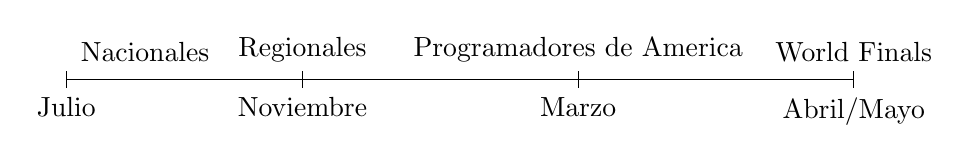
\begin{tikzpicture}
        \draw (1,0) -- (11,0);
        \foreach \x in {1,4,7.5,11}
            \draw (\x cm,3pt) -- (\x cm,-3pt);
            \draw (1,0) node[below=3pt] {Julio} node[above=3pt] {};
            \draw (2,0) node[below=3pt] {} node[above=3pt] {Nacionales};
            \draw (4,0) node[below=3pt] {Noviembre} node[above=3pt] {Regionales};
            \draw (7.5,0) node[below=3pt] {Marzo} node[above=3pt] {Programadores de America};
            \draw (11,0) node[below=3pt] {Abril/Mayo} node[above=3pt] {World Finals};
    \end{tikzpicture}
\end{frame}

\section{Datos del TC}
\begin{frame}{Datos}
    \begin{itemize}
        \item En estas dos semanas van a resolver entre 35-70 problemas.
        \item Desde el 2010, el 95\% de los finalistas argentinos, participaron del TC Argentina.
        \item De los últimos 5 equipos Latam Champions, 4 participaron del TC Argentina.
    \end{itemize}
\end{frame}

\section{Un poco de historia del TC}

\begin{frame}{Los comienzos}
    
    \begin{itemize}
        \item El Training Camp Argentina nace en 2010, inspirandose en los entrenamientos que venian realizandose en Rusia, y que habia comenzado el año anterior en Brasil.
        \item Ese primer Training Camp duro 5 días, y se realizo en la UBA.
        \item Ese primer año solo participaron equipos de Argentina.
        \item Ya al año siguiente se sumaron equipos de países vecinos.
    \end{itemize}
\end{frame}

\begin{frame}{Sedes}
    \begin{itemize}
        \item 2010 - FCEN UBA, Ciudad Autónoma de Buenos Aires
        \item 2011 - FCEN UBA, Ciudad Autónoma de Buenos Aires
        \item 2012 - FAMAF UNC, Ciudad de Cordoba, Cordoba
        \item 2013 - UNLP, La Plata, Provincia de Buenos Aires
        \item 2014 - FCEN UBA, Ciudad Autónoma de Buenos Aires
        \item 2015 - UNS, Bahia Blanca, Provincia de Buenos Aires
        \item 2016 - UNComa, Ciudad de Neuquén, Neuquén
        \item 2017 - UNSAM, San Martin, AMBA, Provincia de Buenos Aires
        \item 2018 - FCEN UBA, Ciudad Autónoma de Buenos Aires
        \item 2019 - FAMAF UNC, Ciudad de Cordoba, Cordoba
        \item 2020 - Remoto
        \item 2021 - Remoto
        \item 2022 - Remoto
        \item 2023 - UNLaM, La Matanza, AMBA, Provincia de Buenos Aires
        \item 2024 - UNR, Rosario, Santa Fe
        \item $\bm{2025 - UTN FRSF, Santa Fe}$
    \end{itemize}
\end{frame}

\section{Universidad Tecnológica Nacional - FRSF}

\begin{frame}{Universidad Tecnológica Nacional}
    \centering
    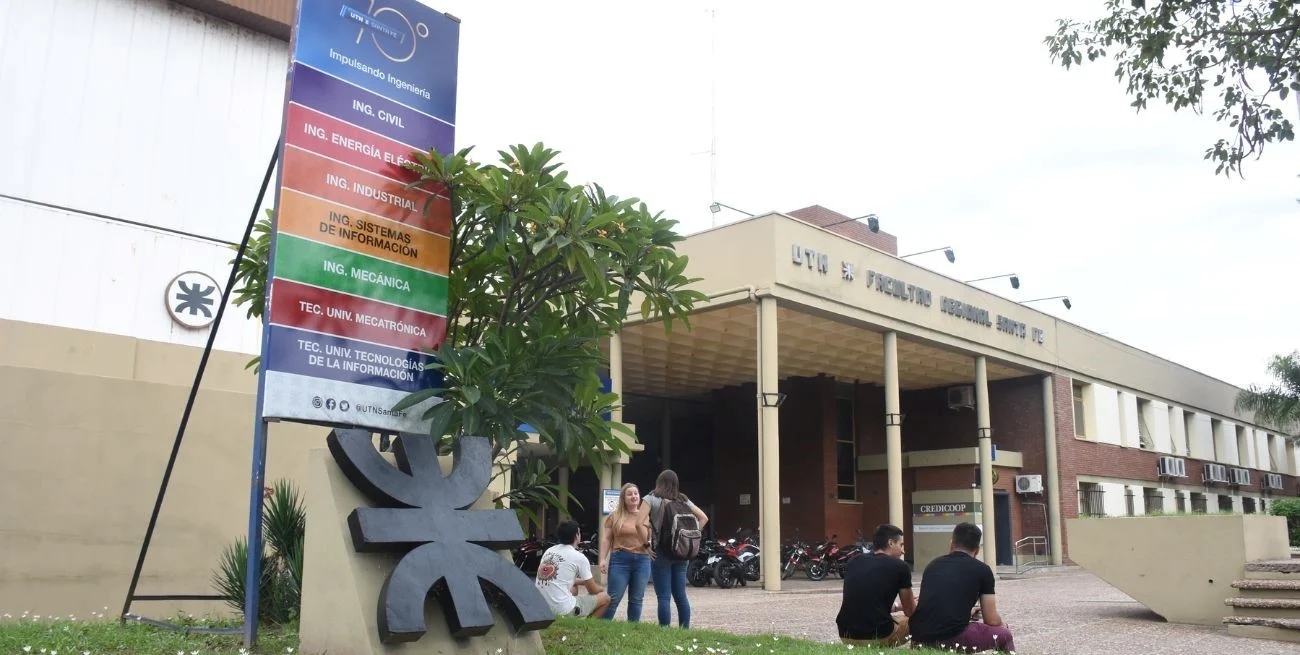
\includegraphics[width=0.8\textwidth]{img/utn_00.png}
\end{frame}

\begin{frame}{UTN FRSF en ICPC}
    \begin{columns}[t]
        \column{0.5\textwidth}
        \centering
        2019 - Porto WF\\
        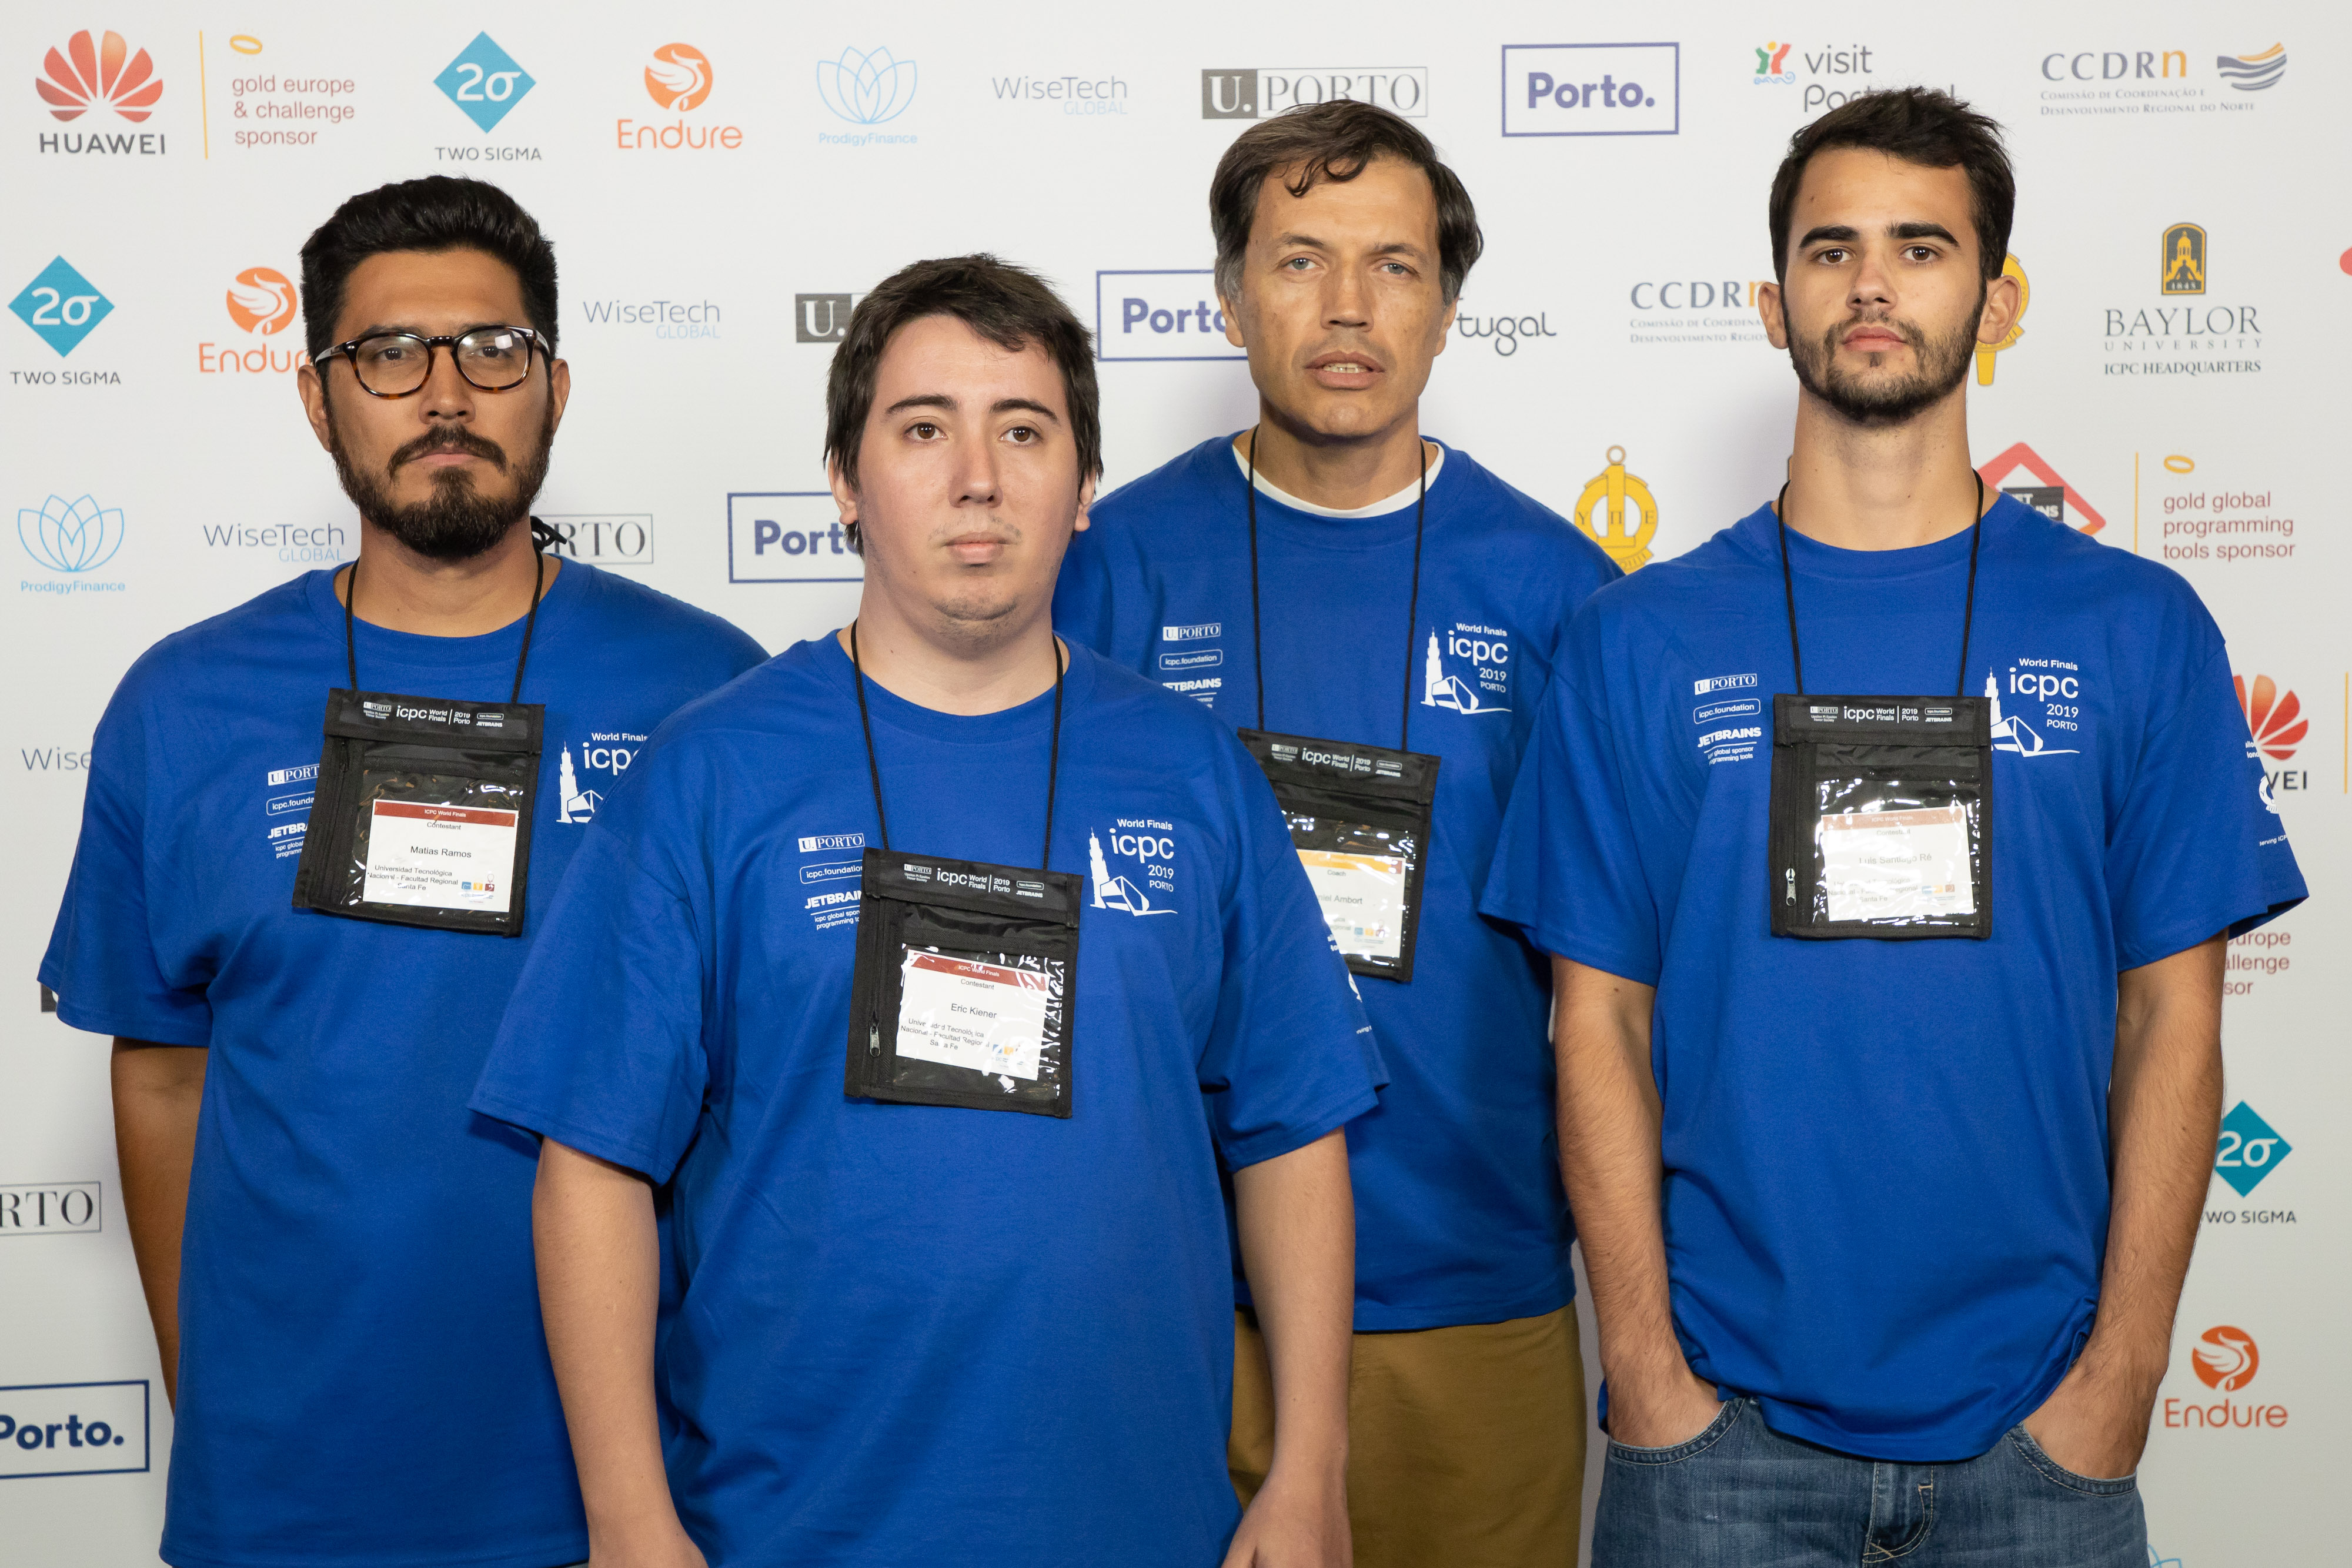
\includegraphics[width=1\textwidth]{img/utn_wf_01.jpg}
        \column{0.5\textwidth}
        \centering
        2019 - Porto WF\\
        \includegraphics[width=1\textwidth]{img/utn_wf_02.jpg}
    \end{columns}
\end{frame}


\begin{frame}{UTN FRSF en ICPC}
    \begin{columns}[t]
        \column{0.5\textwidth}
        \centering
        2022 - Egypto WF\\
        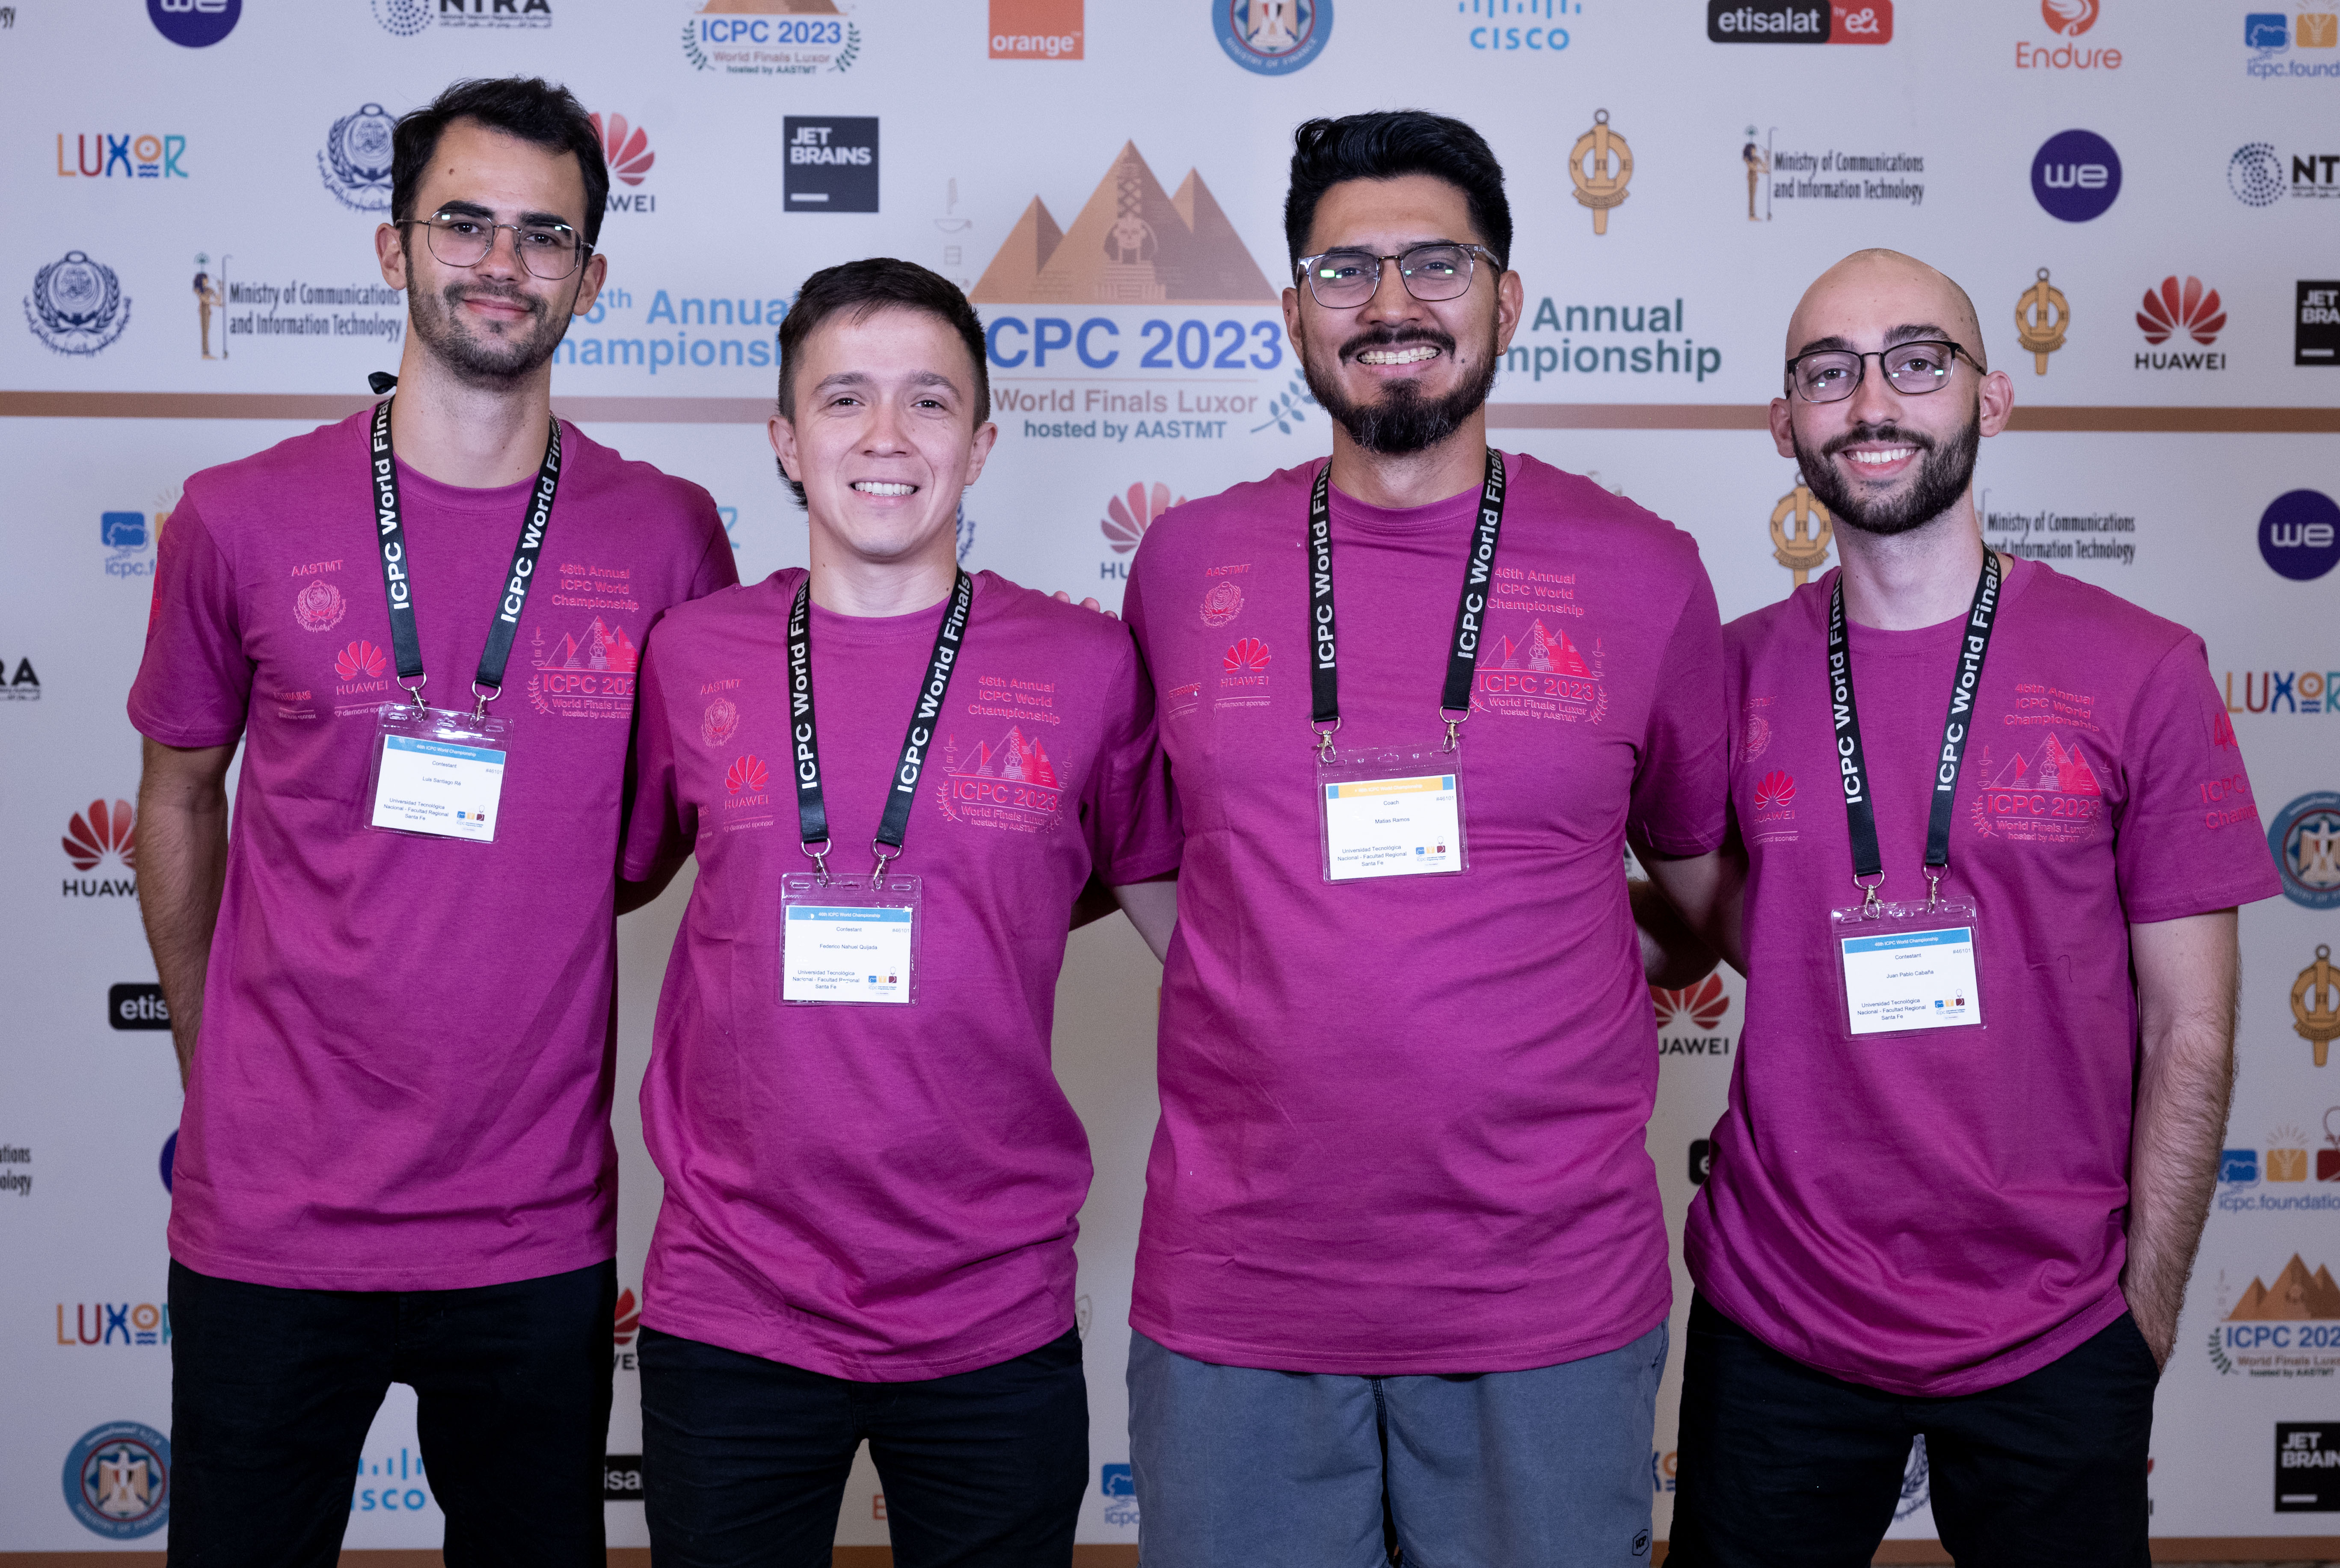
\includegraphics[width=1\textwidth]{img/utn_wf_03.jpg}
        \column{0.5\textwidth}
        \centering
        2022 - Egypto WF\\
        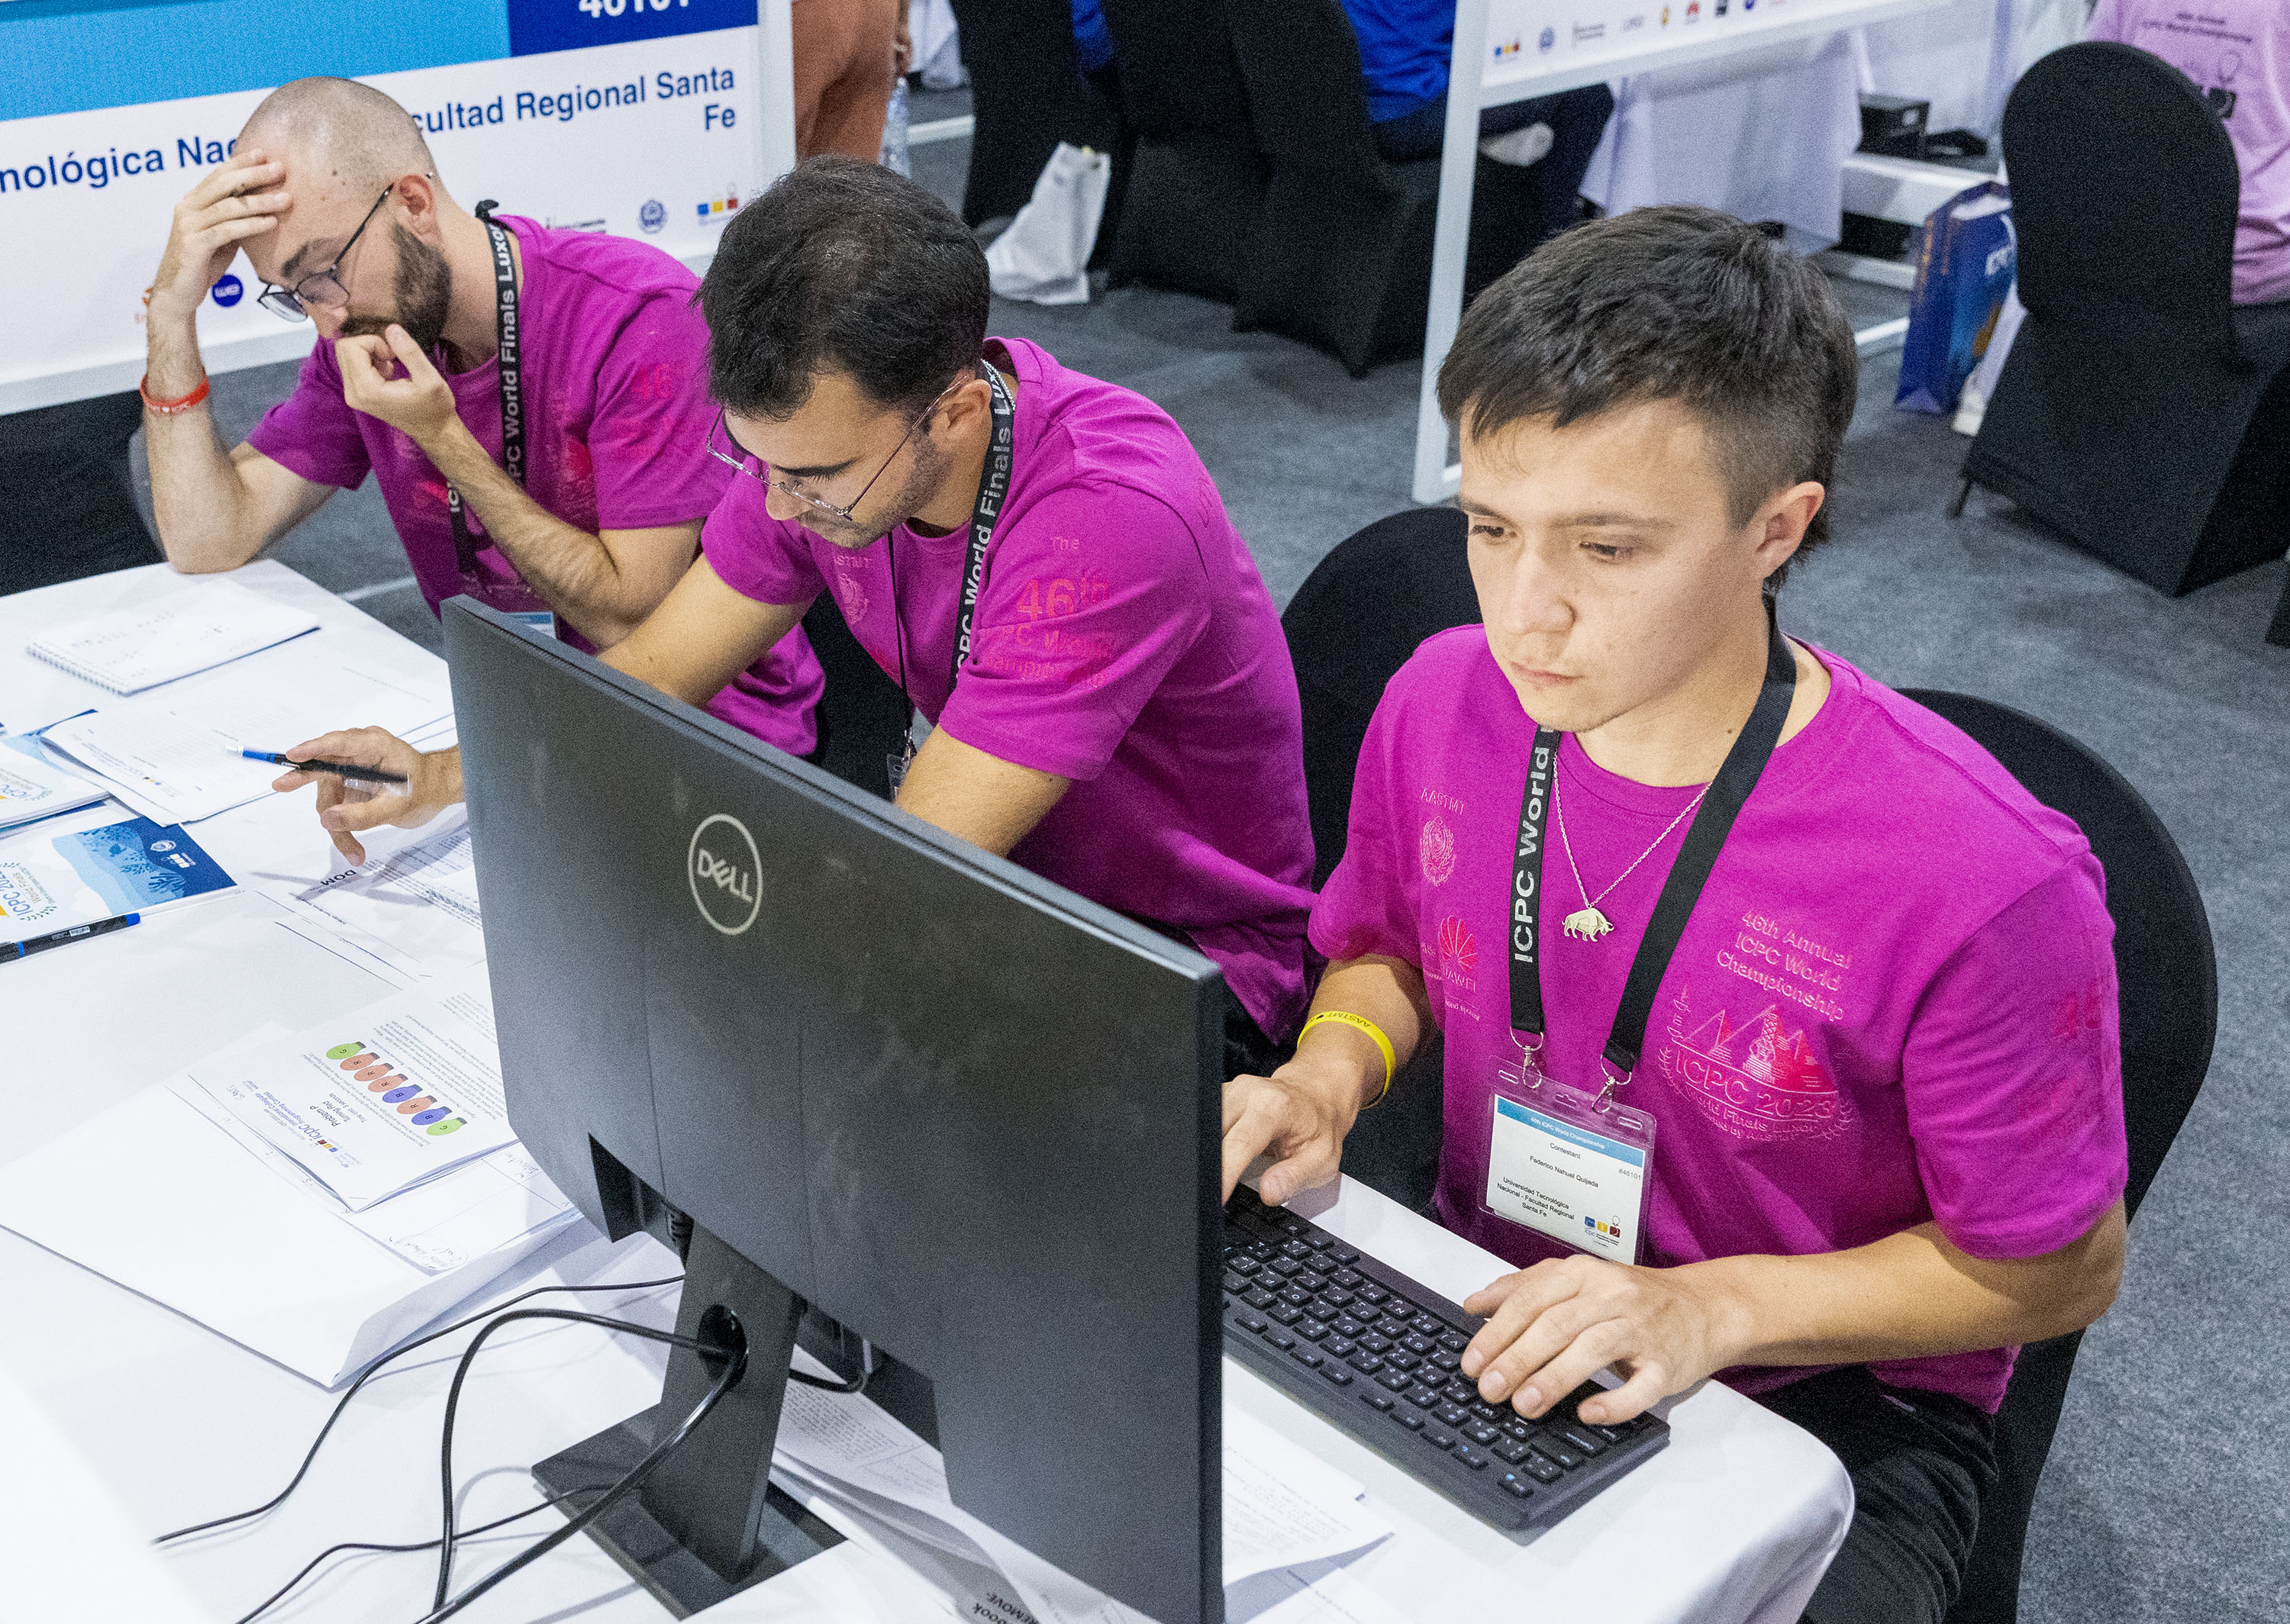
\includegraphics[width=1\textwidth]{img/utn_wf_04.jpg}
    \end{columns}
\end{frame}

\begin{frame}{UTN FRSF en ICPC}
    \centering
    2024 - PDA Guadalajara\\
    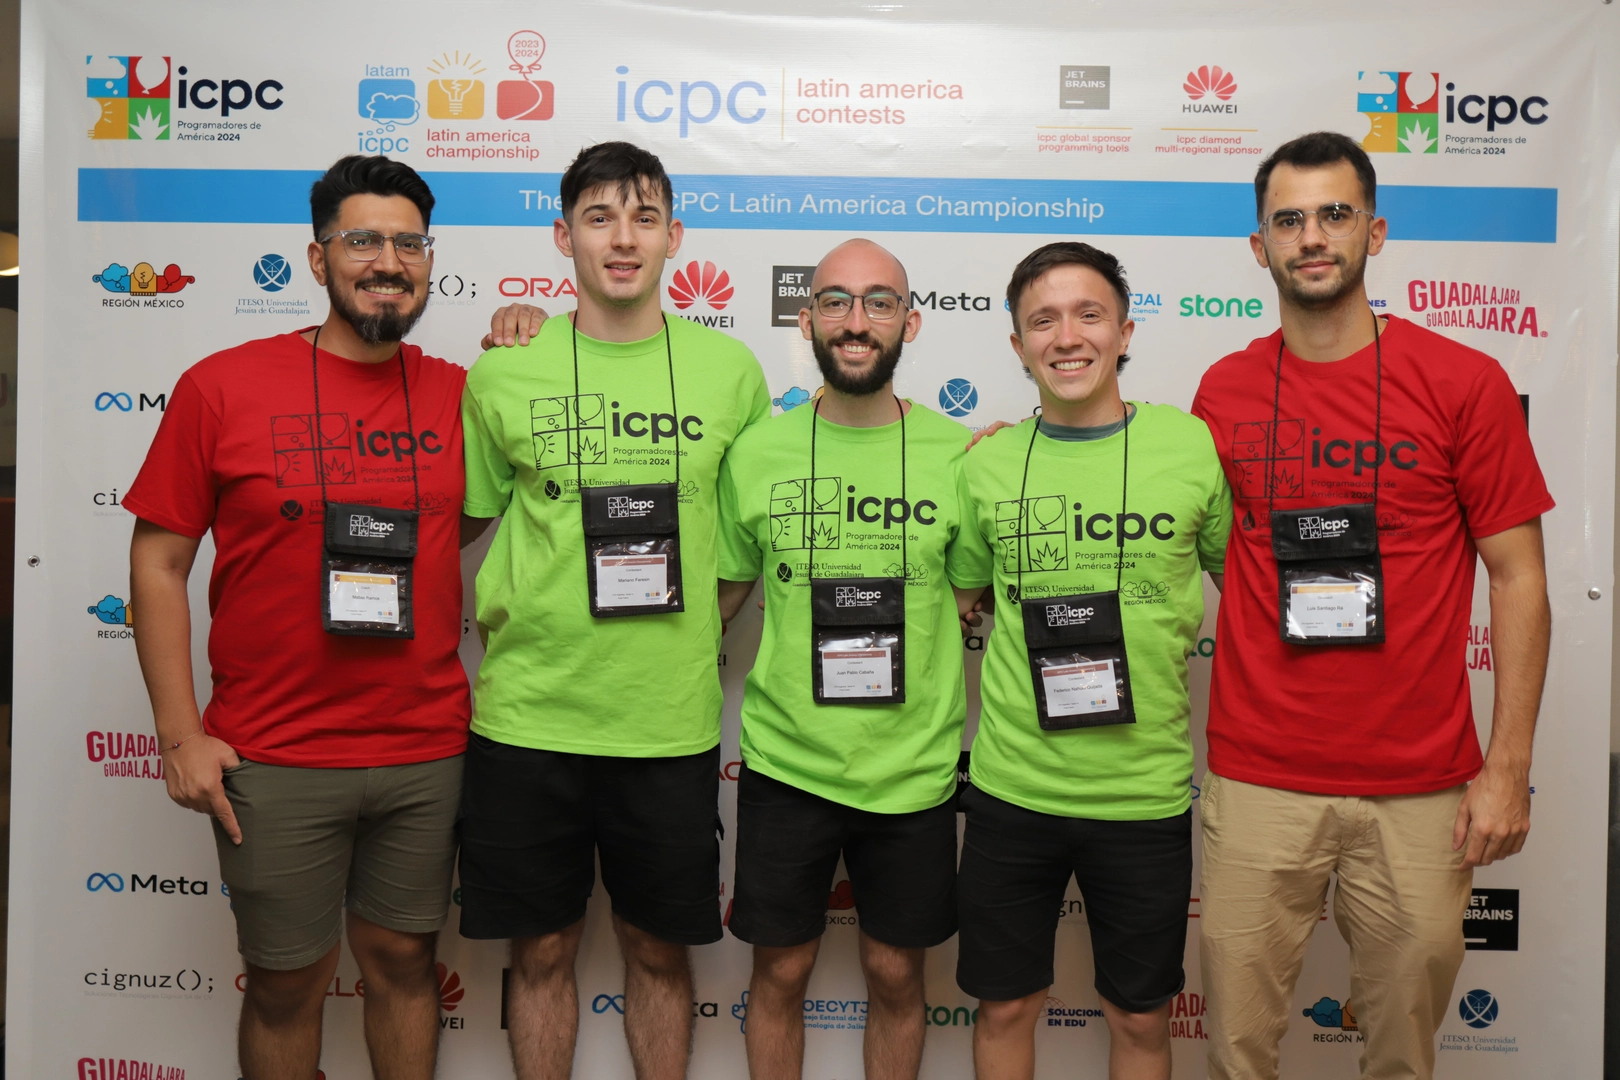
\includegraphics[width=0.8\textwidth]{img/utn_pda_01.png}
\end{frame}

\begin{frame}{UTN FRSF en ICPC}
    \begin{columns}[t]
        \column{0.5\textwidth}
        \centering
        2024 - Kazajstan WF\\
        \includegraphics[width=1\textwidth]{img/utn_wf_05.jpg}
        \column{0.5\textwidth}
        \centering
        2024 - Kazajstan WF\\
        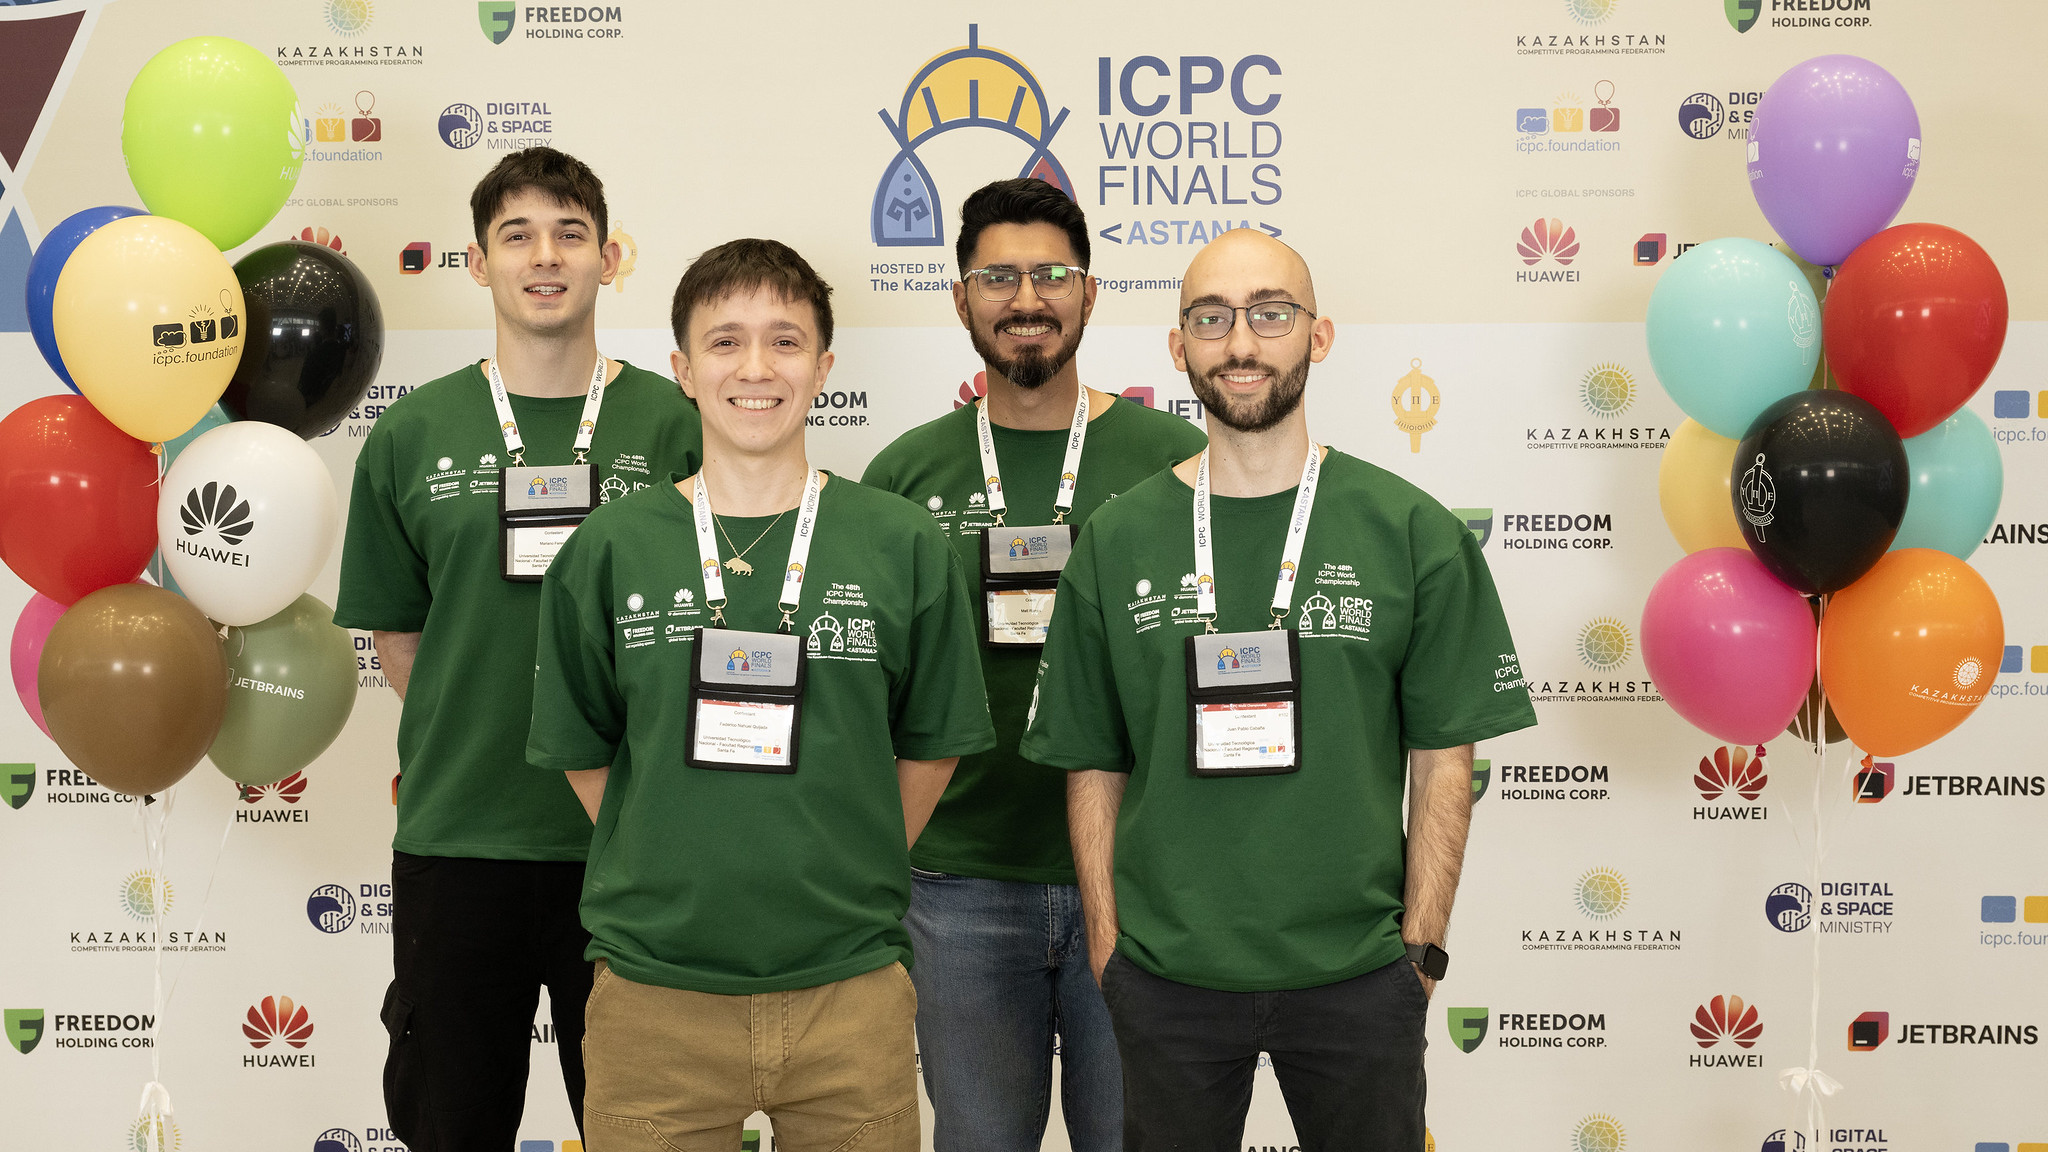
\includegraphics[width=1\textwidth]{img/utn_wf_06.jpg}
    \end{columns}
\end{frame}

\begin{frame}{UTN FRSF en ICPC}
    \centering
    2025 - PDA Bahia\\
    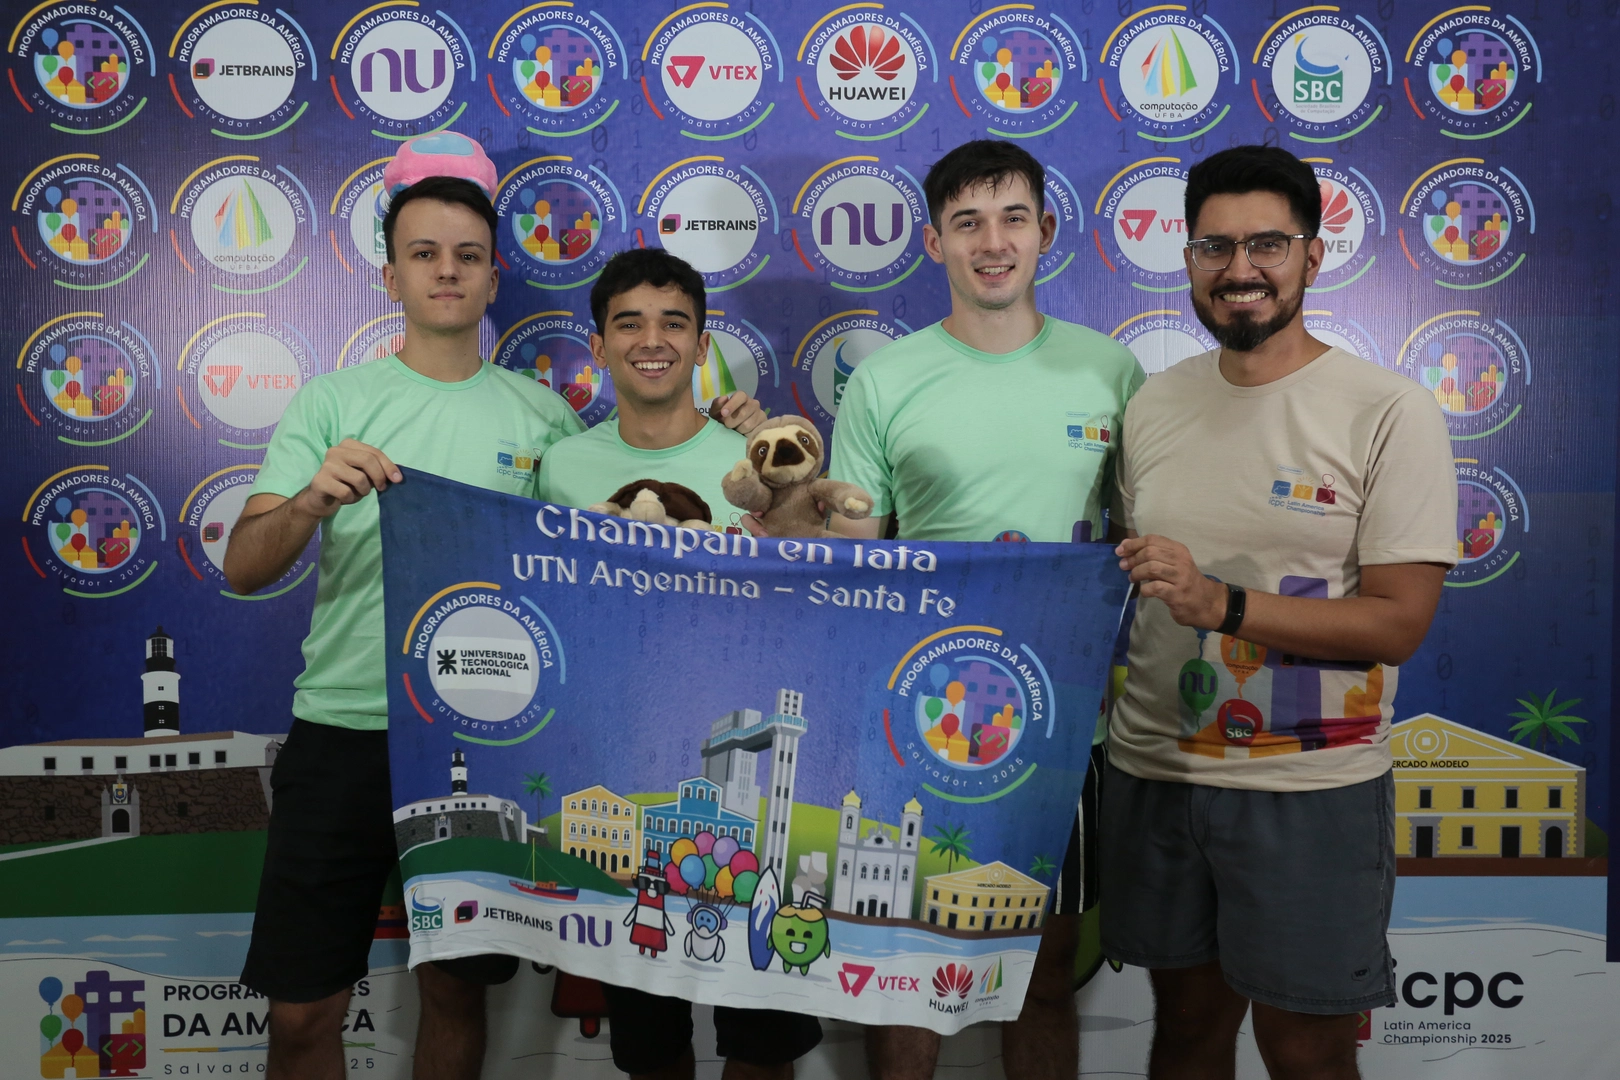
\includegraphics[width=0.8\textwidth]{img/utn_pda_02.png}
\end{frame}

\section{Palabras}

\begin{frame}{Universidad Tecnológica Nacional - FRSF}
    \centering
    
\includegraphics[width=0.8\textwidth]{logos/utn_santafe.png}
    
    \vspace{0.5cm}
    
    Milagros Gutierrez - Directora del Departamento de Ingenieria en Sistemas de Información
\end{frame}

\begin{frame}{Gobierno de Santa Fe}
    \centering
    
\includegraphics[width=0.8\textwidth]{logos/santa_fe_logo_v2.jpg}
    
    \vspace{0.5cm}
    
    Erica Hynes - Secretaria de Ciencia Tecnología e Innovación
\end{frame}

\section{Cronograma}

\begin{frame}{Día Inaugural}
    Usted está aquí
    \centering
    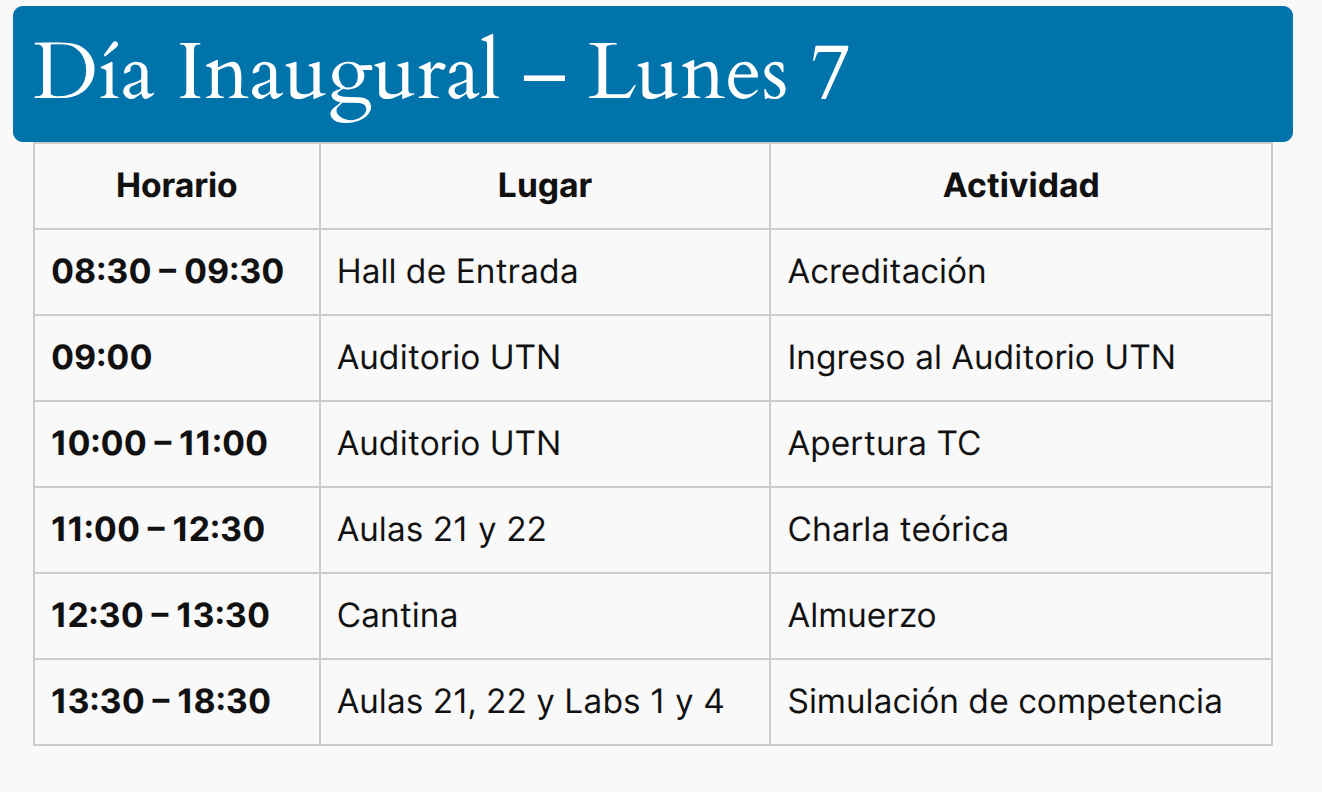
\includegraphics[clip,height=7cm,keepaspectratio]{img/crono_01.png}
\end{frame}

\begin{frame}{Almuerzo}
    \centering
    El almuerzo es de {\bf 12 a 13:30 hs}, el horario se respeta siempre.
    
    {\bf No lleguen tarde.}
    
    \vspace{0.5cm}
    
    Puede llegar antes. Seamos ordenados que el espacio en cantina es limitado. Se pueden usar las mesas en el hall de entrada.
    
    {\bf *Seamos limpios*}
\end{frame}

\begin{frame}{Día GTS}
    \centering
    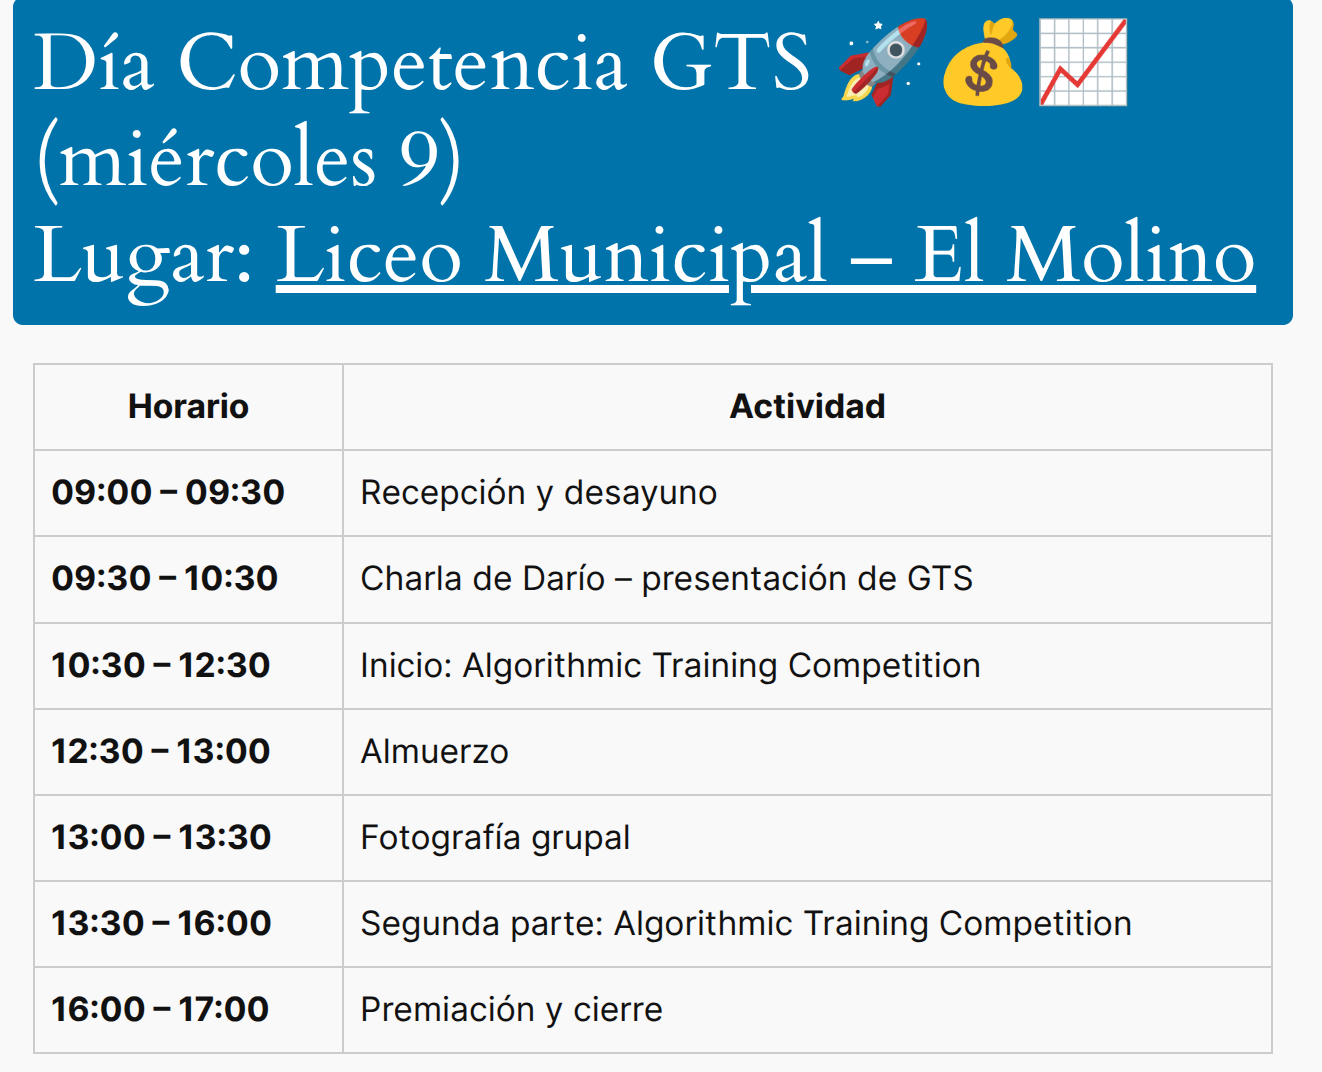
\includegraphics[width=\textwidth,height=\textheight,keepaspectratio]{img/crono_02.png}
\end{frame}

\begin{frame}{Días normales}
    \centering
    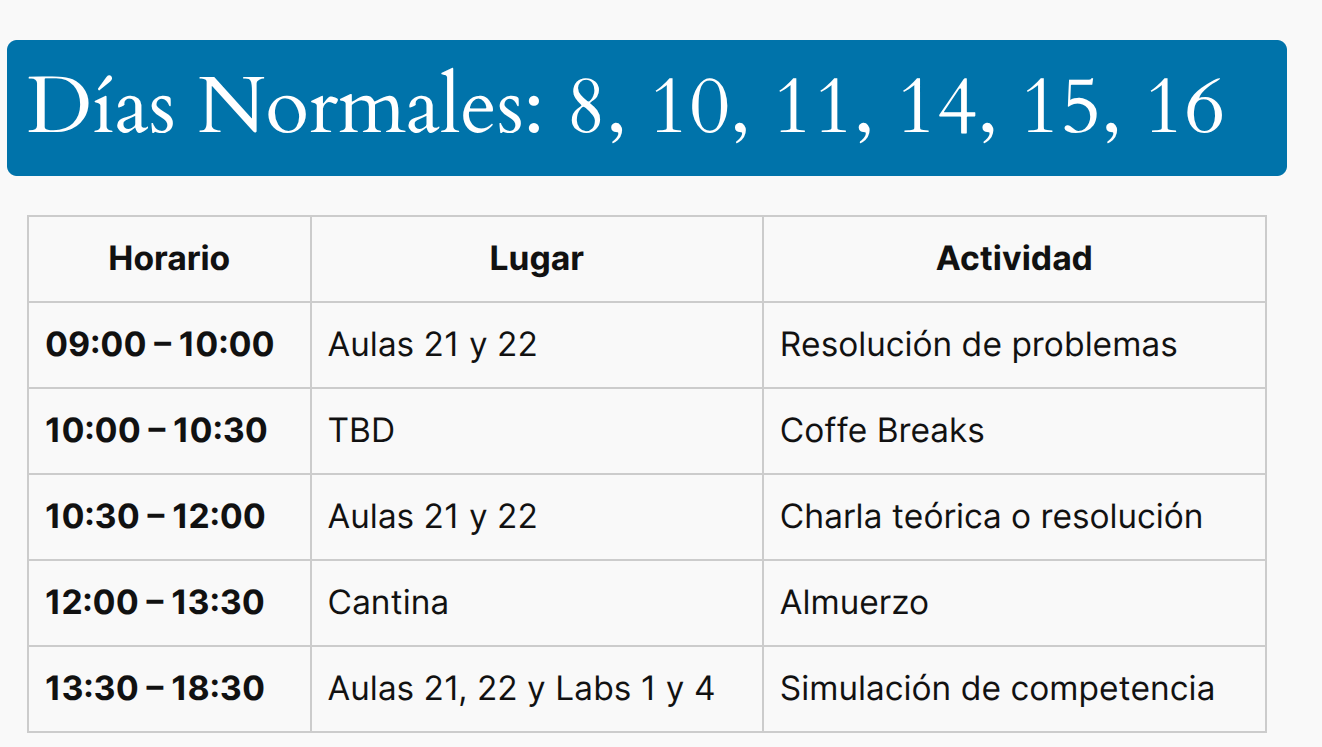
\includegraphics[clip,height=7cm,keepaspectratio]{img/crono_03.png}
\end{frame}

\begin{frame}{Días Sponsors Gold}
    \centering
    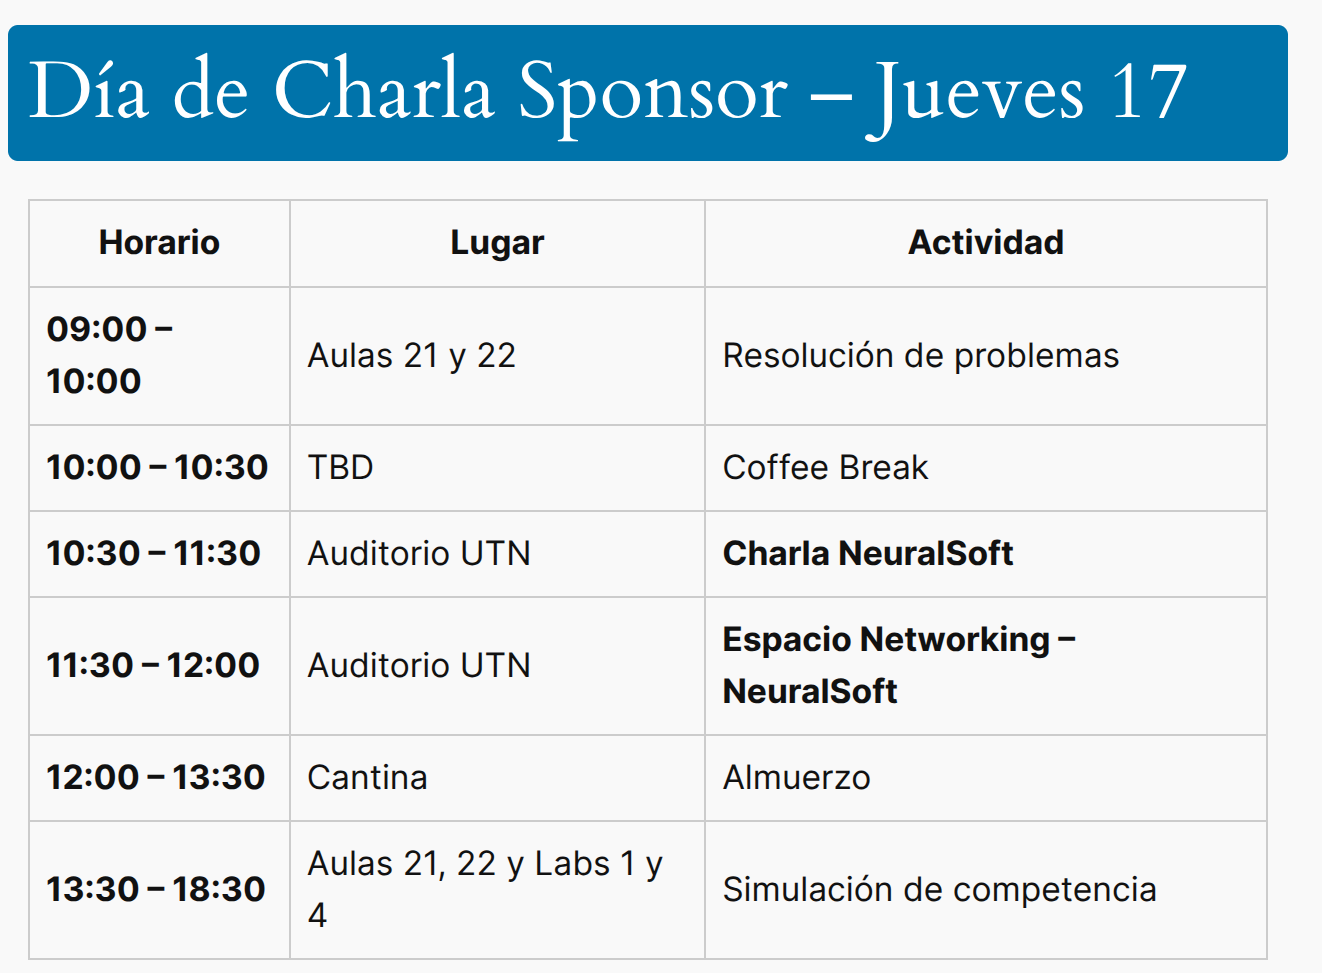
\includegraphics[clip,height=7cm,keepaspectratio]{img/crono_04.png}
\end{frame}

\begin{frame}{Día de Cierre}
    \centering
    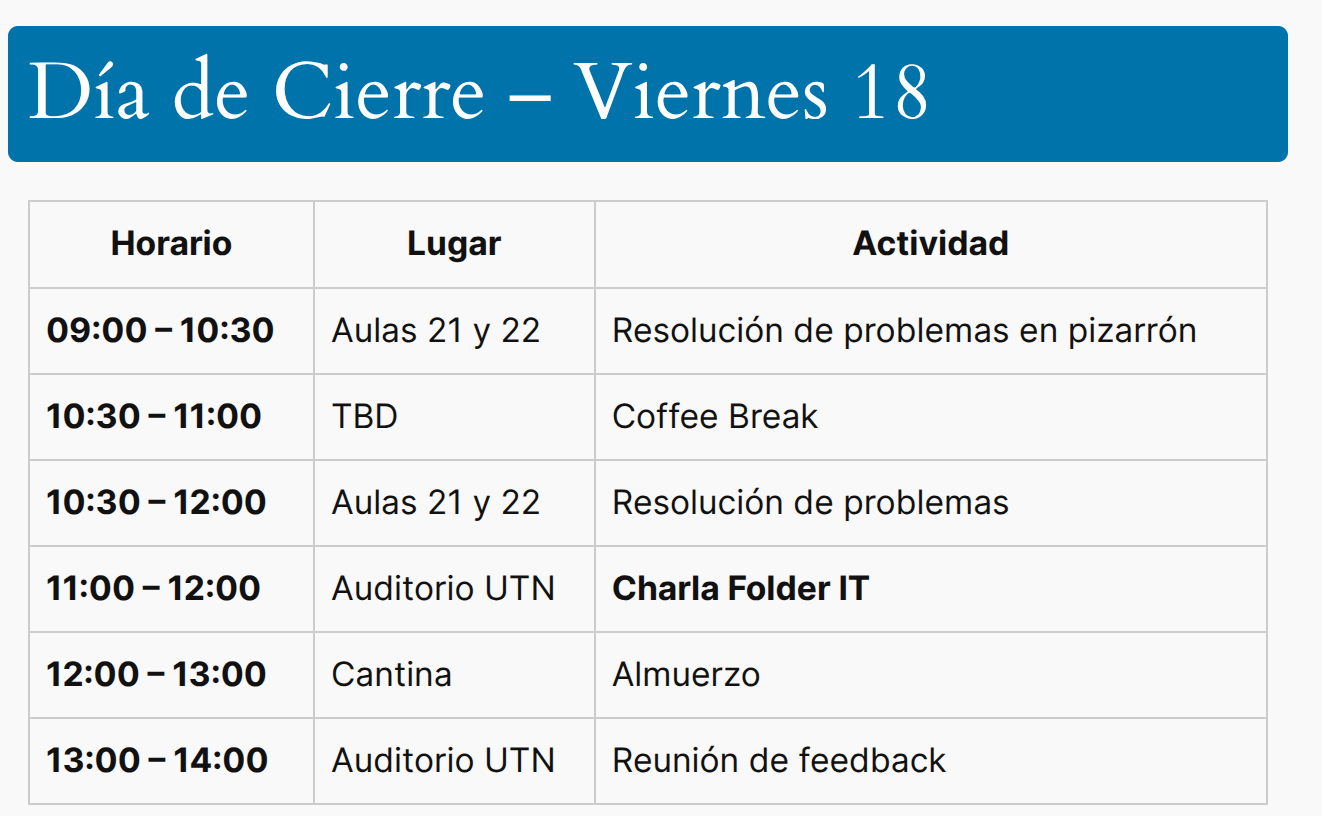
\includegraphics[clip,height=7cm,keepaspectratio]{img/crono_05.png}
\end{frame}

\begin{frame}{Aulas y espacios}
    \centering
    {\bf Aulas 21 y 22}
    
    \vspace{1cm}
    
    Para simulaciones:
    \begin{itemize}
        \item Laboratorios 1 y 4
        \item Se pueden utilizar las aulas 21 y 22 con notebooks personales
    \end{itemize}
\end{frame}

\begin{frame}{Dudas}
Para dudas o consultas pueden:
        \begin{itemize}
            \item Contactar al Staff (voluntarios u organizadores)
            \item Preguntar por el grupo de Telegram
        \end{itemize}
        %\bibliography{ref}
\end{frame}

\begin{frame}{Gracias}
    \centering
    Gracias a todos por venir.\\
    Suerte en la competencia de hoy!
\end{frame}


\end{document}